% This is LLNCS.DEM the demons\textbf{}tration file of
% the LaTeX macro package from Springer-Verlag
% for Lecture Notes in Computer Science,
% version 2.4 for LaTeX2e as of 16. April 2010
%
\documentclass{llncs}
%
\usepackage{makeidx}  % allows for indexgeneration
\usepackage{CJKutf8}
\usepackage{graphicx}
\usepackage{authblk}
\usepackage{verbatim}

\begin{document}
\title{Natural Language Processing for Social Event Classification}
%
\titlerunning{NLP for SEC}  % abbreviated title (for running head)

\author{Duc-Duy Nguyen\inst{1}, Minh-Son Dao\inst{1} \and Truc-Vien T. Nguyen\inst{2}}
\institute{University of Information Technology\\ Vietnam National University HCMC, Vietnam \\
\texttt{nguyenduy.uit@gmail.com, sondm@uit.edu.vn} 
\and
University of Lugano, 6900 Lugano, Switzerland \\
\texttt{thi.truc.vien.nguyen@usi.ch}
}

\maketitle
%

%
%\title{Natural Language Processing for Social Event Classification}
%
%\titlerunning{NLP for SEC}  % abbreviated title (for running head)
%                                     also used for the TOC unless
%                                     \toctitle is used
%

%

\begin{abstract}
In this paper, a simple but effective method for social event detection based mainly on natural language processing is introduced. Meanwhile existing approaches use many typical text-classification methods and disregard the importance of language characteristics, the proposed method exploits such language characteristics from text items in social metadata (e.g. title, description and tag) to leverage social event detection. First and foremost, we analyze the specific characteristics of natural language in social media to choose the most suitable features. Second, we employ common natural language processing techniques along with machine learning methods to extract features and perform classification. As a result, we experienced the F1 score higher than the results of related works that used state-of-the-art methods. The proposed method proves the significance of understanding language characteristics in building social event classification programs. It also offers good clues to improve existing works on social event detection.

\keywords{Social Event Classification, Social Event Detection, social network, text classification, language processing, natural language characteristics}
\end{abstract}
%
\section{Introduction}
%
Just within decades, we have witnessed the dramatical development of social networks (SNs) where users can share their data and interact with their's friends data easily and quickly.  For example, Facebook\footnote{www.facebook.com}, Twitter\footnote{www.twitter.com}, LinkedIn\footnote{www.linked.com}, Instagram\footnote{www.instagram.com}  comfort their users very well with various and attractive features such as personal information sharing (create, update, public profiles), media creation and sharing (message, photo, video, file. etc.), personal network management, applications. These advantages bring SN a unique ability to connect billions of users worldwide and establish online communities where user connected each other by friendship \cite{ellison2007social}. 

The interesting research presented in \cite{kwak2010twitter} reveals the fact that media content from SNs can effectively reflect the problems or events, since majority of topics are headline news or message from famous people/organization. Beside, recent researches concern with a possibly next generation of SN known as Social Life Network (SLN)[8], inspired by the idea of connecting people and their interested resources. Specifically, SLN helps people not only connect to each other and sharing experiments, but also provide them to efficient means to keeping up with real-time and real-life resource (many of whom come under the form of events). Therefore, there is a tight relation between social data and events they represent for. 

This dramatically increases an emergent demand of controlling social media resources to facilitate the evolution of SN and user-centric web technology \cite{kwak2010twitter}. Obviously, social event classification play an undeniable importance in detecting, organization and mining events, not only to the SN today, but also to the future of SN. Therefore social event detection has become a hot topic within a decades. In \cite{reuter2013social}, social event is defined as follow: \textit{“the events that are planned by people, attended by people and for which the social multimedia are also captured by people.”}. That leads to the trend of analyzing social media to understand social events. 

Since many social media contents today come with accompanying metadata (time-stamps, tags, geographic tags, uploader’s ID, etc.), these information itself partially reflects the insight of the contents. Therefore, we point our target to exploit tag and title to show how effective they are on solving social event classification problem. 

To tackle the challenges, we consider SEC as a supervised text classification problem. First of all, we specify the characteristics of the Social Media natural languages and explain how it affects the performance of many typical text classification methods. Second, we proof our arguments by proposing a method based on Social Media characteristics. 

We select features based on characteristics of Social Media natural language. Then we extract selected features using common Natural Language Processing tools. After that, we use a bag-of-words like model for simplifying representation metadata of a media content before employing Support Vector Machine as supervised learning method. For experiments, we apply our methods to MediaEval 2013 dataset \cite{reuter2013social} for Social Event Detection since it is an up-to-date dataset from a populated SN. For evaluation, we use F1 score from precision and recall as evaluation metric.

\textbf{Contribution}: One of the most significant characteristics of SNs is free-style text contents. SNs is known as the place where users can be unique by using their own styles. Therefore, languages used in SNs differs from normal language used in real world. Unfortunately, many existing works apply complex text classification technique on solving SEC did neglect or pay less attention on characteristics of social media natural language. Therefore, the proposed method tries to explore and exploit these characteristic to increase the accuracy of social event detection as well as the speed of processing stage in order to cope with real-time processing requirements. 

\section{Related Works}

In \cite{itikavit}, the authors compute semantic relatedness between the synset representing the tags and each of the categories. They used Lin – a WordNet-based relatedness similarity measure proposed by Dekang Lin in \cite{lin1998information}. Lin measure bases on information content of the least common subsumer (LCS). It sums the information content of the individual concepts then scale this sum; the result is the information content of the LCS. For those media contents that encounter the same Lin measure result, they use another constrain (Date, Time) to determine the best result. This method gain the event F1 score $7.48\%$. The method represented in \cite{schinas2012certh} give the F1 score of $22.01\%$ of even/non-event classification. This method first used 1000 most frequent tags then applied 200 latent topics as features. The concept of which the detector produced the highest prediction score is assumed to be the choice. 

Another team employs machine learning models for supervised learning and classification. In \cite{brenner2012social}, the authors uses title, description and keywords of metadata to build classifier for each event type. They employed linear \textit{support vector machine} classifier to classify test samples. Instead of classifying media content individually, they first apply constraint-based Spatiotemporal clustering to cluster media contents, then apply classification on groups of items. This method gained F1 score $37\%$. The best methods for social event classification from metadata is reported in \cite{daoICMR14}, where the authors extracted the following features from text of title, description and tag: original word, word in lower-case, prefixes, suffixes, part-of-speech, orthographic characteristics and ontological feature. They also employed \textit{support vector machine} as supervised machine learning method and \textit{disambiguation} to Wikipedia\footnote{www.wikipedia.com} to optimize the performance. As a result, they experimented the F1 score $47.61\%$.

All the above works used typical text classification technique. They treat text from SN normally, no clear-concern over characteristics of natural language in Social Media. In addition, many of these techniques \cite{schinas2012certh} \cite{brenner2012social} \cite{sakaki2010earthquake} are complex and require much time and resources, therefore they are not applicable for real-time applications. 

\begin{figure}[tb]
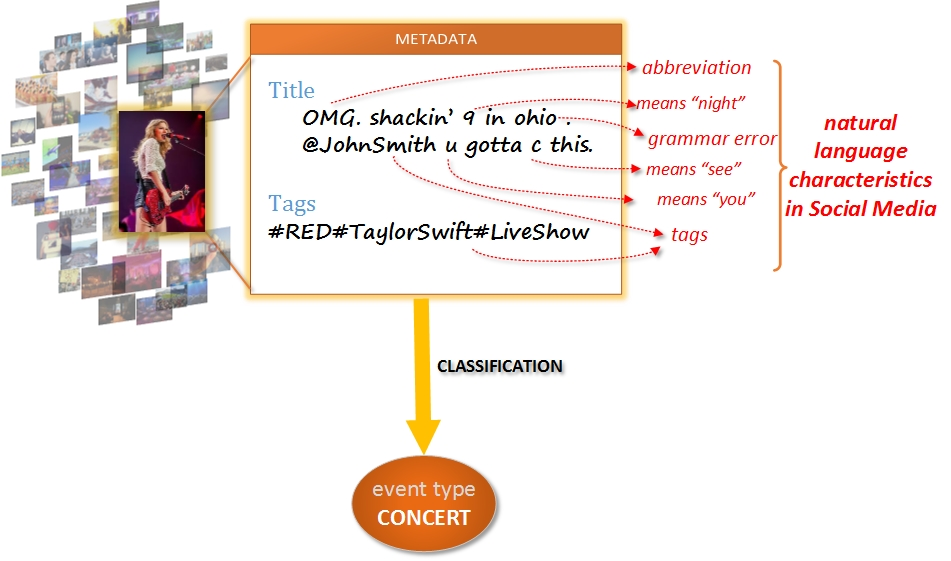
\includegraphics[width=12.0cm, height=8.0cm]{fg1.jpg}
\caption{Social Even Classification on natural language of Social Media}
\end{figure}

\section{Methodology}

The proposed method focuses on understanding the characteristics of Social Media natural language (verbal) and apply these characteristics on proposing a simple and effective method to solve SEC problem. In section \ref{NLPSM}, we discuss characteristics of Social Media natural language from causes to effects. In section \ref{Features}, we show how we apply these characteristics on text feature selection. In section \ref{BoW}, we represent our document representing model and the learning model that we used to build the classifier. 

\subsection{Natural language characteristics in Social Media }
\label{NLPSM}

Language is an interactive and social phenomenon that centralize to the inter-personal communication between individuals in a society \cite{duranti1992rethinking}. Thus, language is always dynamically affected and evaluated with the changes of its society. In SN, its cross-culture and up-to-date environment push the evolution of language obviously. In this section, we turn our attention to find out the characteristics of English language which is widely used by SN users. There are many factors that make up the characteristics of social media natural language today. Five main factors are concerned as follow:

\begin{itemize}
\item \textbf{Fast and short message composing habit}: modern mobile internet technologies and smart devices such as smartphone, tablet PC, etc., are providing fast and convenient methods that help people are easily connected to SNs anywhere. For instance, a man can visit Facebook when he is in the elevator, waiting for the bus. Their messages, often short and impact, contain many words under shortened form, slang or novel words. In addition, some SNs limit the maximum number of character of the message, for instance, Twitter set tweet maximum number of character to 140, hence, users have to constrict their message and discard grammar rules and unimportant words.

\item \textbf{Young users’ ages}: a research by Pew Research Center (PRC) shows that by September 1st 2013, $90\%$ of online American adult ages 18 -29 are SN users. For adult ages 30-49 and 50-64, $87\%$ and $65\%$ of them do, respectively. An earlier PRC research reveals that $81\%$ of American online teens use some kind of SN by September 2012. These statistics could by different by country and time, however it show that a great number of young people are using SN everyday. Notably, these young user often use slang and informal words in their communication; thus the text in Social Media today contain lots of noises.

\item \textbf{Open and multicultural environment}: SNs attracted billions of people who came from different societies, have different educational backgrounds, speak different languages and interest in very different things. This make SN become a multicultural environment, especially the language usage. 

\item \textbf{From anonymity, equality to freedom}: Anonymity is one of the most important characteristic that SN inherited from its ascendant - the internet. Specifically, a person can partly hide his/her real identify; or reveal things that they want other people think he/she is. In addition, SN provide an environment where people can equally express their ideas, no matter who they are. These two characteristics give the users the feeling of freedom, hence many people quickly express their ideas without caring about language mistakes.

\end{itemize}

The above factors make up characteristics of language in social media, included:

\begin{enumerate}
\item \textbf{Lots of Noise}: many words in Social Media are dialect or meaningless.
\item \textbf{Abnormal vocabulary}:
\begin{itemize}
\item \textbf{English-based Creole Languages}: words that derive from English languages. For example: in Singlish (i.e. colloquial Singaporean English) the word \textbf{then} often be written or pronounced \textbf{den}; or in Hawaiian Pidgin English the word \textbf{baby} often be replaced by \textbf{behbeh}.

\item \textbf{High Diversity}: The diversity of English in social media come from it multi-cultural environment. As a result, (1) English slang and “half-English” slang are widely used. For example, the English slang \textbf{“Lose The Plot”} means to go crazy or suffer mental illness. Also, there are some special English slang which combine an alphabet character and a non-English character/word, (2) Multilingual environment allows user to use their own language and vocabulary, and (3) Many abbreviation are used. Such as in Figure 1, the word \textbf{OMG} is abbreviation of “Oh my God!”.
\end{itemize}

\item \textbf{Abnormal Grammar}
\begin{itemize}
\item \textbf{Weak Grammar Constrains}: As we mentioned early this section, fast and short message composing habits make user dismiss or misuse grammatical rules, such as capitalize proper nouns, tense, punctuation marks usage, etc.

\item \textbf{Specific Structures}: There are some considerable sentences that we can see everywhere on SN, such as “Like us on Facebook.”, “Forgot your password?” or “Ask me anything!”. These specific sentences focus on easy to understand and remember, therefore the structure was simplified, often violate common grammar rules.

\end{itemize}

\item \textbf{Other Characteristics}:
\begin{itemize}
\item \textbf{Hashtag}: indicates the topic/category of the post.
\item \textbf{At-tag}: indicates another user.
\item \textbf{Emotion}: such as “:)”, “:b”, “(:”, etc.

\end{itemize}
\end{enumerate}

\subsection{Feature selection based on characteristics of natural language in Social Media}
\label{Features}

Based on characteristics that explained in section \ref{NLPSM}, we come with three assumptions:

\begin{enumerate}
\item The dictionary or list of words on which feature extraction carries out must be very rich. Ideally, it should be an independent dictionary consist all English and Non-English words, slang, aberration, dialect, etc.. A too small dictionary (such as the work \cite{schinas2012certh}) could lead to low effective feature representation. However, at the moment, there are no such a perfect dictionary; so the alternative choices could be conducting the dictionary from the training data itself to get as many words as possible. Therefore, a bag-of-word like model could be a good choice.

\item Many grammar-related features, such as parse tree, do not work effectively on social media language, due to its abnormal grammar.

\item For statistics approach, words should be transform into its base form to fill the gap between differences. The diversity as explained in \ref{NLPSM} comes from abnormal vocabulary or error on grammar need to be considered. For example, words \textbf{car, cars, car's, cars', Car, CAr} should be understand as \textbf{car}. Without this step, all the words will be treat individually, therefore no similarity between them can be seen. This is also an important step before applying Similarity compute using a dictionary/knowledge-based like WordNet\footnote{wordnet.princeton.edu}. Discarding this step may lead to the low performance problem en-countered by \cite{itikavit}, because all term that is not under the base form can not be found in WordNet. Likewise, the above problem also limited the effectiveness of ontology extraction \cite{daoICMR14}.

\end{enumerate}

The above assumptions help us propose a simple but suitable set of text features, included:

\begin{enumerate}
\item $w_{i}$ the original word in title, description or tag of the metadata.
\item $lc_{i}$ is $w_{i}$ in lowercased form.
\item $le_{i}$ is base form of $w_{i}$, after applied lemmatization.
\item $ne_{i}$ is the named-entity recognition(NER) result of $w_{i}$. It determines whether $w_{i}$ indicates time, location, organization, person, money, percent, date or other.
\item $p_{i}$ is part-of-speech-tag of the word $w_{i}$, using Penn TreeBank tag set \cite{marcus1993building}.
\item $or_{i}$ is orthographic characteristic of the word $w_{i}$, this determine whether the word is all upper-cased, initial letter upper-cased, all lower-cased or others.

\end{enumerate}

Beside, we use a stopword list from \cite{lewis2004rcv1} to eliminate valueless words. For instance, the word data could be extracted according to our features. In this case, $w_{i}$ is data, $lc_{i}$ is data, $le_{i}$ is datum, $ne_{i}$ is $O$ (means other),  $p_{i}$ is NNS, and  $or_{i}$ is $ALL\_LOWER\_CASED$.

Within the proposed features, the use of feature 1 indicates that we consider all the word in text, feature 2, 3, 4  support our assumption of transforming the word into general or base form, and while feature 5, 6 help us extract basic grammatical features in  weak grammar constrains.

\subsection{Bag-of-words like model}
\label{BoW}

In section \ref{NLPSM}, we explained the abnormal grammar in social media natural language, included weak grammar constrains. Obviously, a sentence with weak grammar constrain accompany with various tags is very similar to an orderless set of words. Therefore, we reuse with some modification the idea of bag-of-words, a model represented by Salton $\&$ McGill in 1983 as a model for orderless document representation.

\paragraph{Bag-of-words Model}: 

Bag-of-words (BoW) is a model for representing document (a sentence, a document) using frequencies of words from a dictionary. BoW is very effective to represent documents, and it completely disregards the order or structure of the words. For example, we have two document. Document 1 is “He bought a new car.” and Document 2 is “He loves his car. She loves it too!”. The dictionary is now contain 10 words that structured as:

\textsf{\{
"He": 1, 
“bought”: 2,
“a”: 3,
“new”: 4,
“car”: 5,
“loves”: 6,
“his”: 7,
“she”: 8,
“it”: 9,
“too”: 10
\}	}

Then document 1 and document 2 represent by the vector [1,1,1,1,1,0,0,0,0,0] and [1,0,0,0,1,2,1,1,1,1], respectively.

\paragraph{The Proposed BoW-like Model}:

In order to use up the advantages of traditional BoW model, we reused its idea, but for multi-dictionaries. That is, we concatenate the vectors representing the document by each dictionary to make the only feature vector for the whole document. We built six dictionaries from training data, they are:

\begin{itemize}
\item \textbf{Original word dictionary}: contains all words of documents in training data.
\item \textbf{Lowercase word dictionary}: contain all words of documents in training data under the form of lowercased.
\item \textbf{Base word dictionary}: contains base form of all words of documents in training data.
\item \textbf{NER dictionary}: contains all NER results: “TIME”, “LOCATION”, “ORGANIZATION”, “PERSON”, “MONEY”, “PERCENT”, “DATE” and “OTHER”.
\item \textbf{Part-of-speech tag dictionary}: contains 40 Penn Treebank Part-of-speech tag appear in training data.
\item \textbf{Orthographic dictionary}: contains orthographic feature: “ALL\_LOWER\_CASED”, “ALL\_UPPER\_CASED”, “INITIAL\_LETTER\_UPPER\_CASED” and “OTHER”.

\end{itemize}

The document is represented by using each of the above five dictionaries, then concatenating the result to have the final feature vector of the document.

\paragraph{Support Vector Machine}:

Support Vector Machine (SVMs) is a highly successful supervised learning model represented by V.N. Vapnik in  \cite{vapnik2000nature} \cite{vapnik1998statistical}. It based on Structural Risk Minimization principle that represented Vapnik in 1995. In \cite{joachims2001statistical}, Joachims also proved that SVMs are very suitable for the solving text categorizing, from both theoretical and empirical approach. Therefore, we employ SVM as supervised learning models for solving our problem. We use linear SVM and optimize parameter with the validation set. Finally, we get the best performance at \textbf{C} (the trade-off between training error and margin) values $2^{15}$.

\section{Experimental Results}
\label{result}

The purpose of experiments is to verify the effectiveness of the approach that a good concern over natural language of Social Media is important to solve SEC problem. We use the dataset, evaluation method and compare the result to the works at MediaEval 2013 \cite{reuter2013social}. MediaEval is a benchmarking initiative, whose reputation is widely accepted by the research community. Its datasets for tasks are updated every year and it uses many standard measurement for evaluation results.

\paragraph{Dataset}: We use the dataset from MediaEval 2013 because it is up-to-date and was collected from Instagram, one of the most popular SN today. The training set included 27,754 pictures, which was collected from $27^{th}$ and $29^{th}$ of April 2013. The test set was collected from $7^{th}$ and $13^{th} $of May 2013 consist of 29,411 pictures. The picture came with some of metadata, but not all. 

\paragraph{Evaluation Tools}: We evaluate our result with the ground truth  annotated manually by MediaEval 2013. We use standard F1-Score from Precision and Recall as evaluation measure. Precision and Recall are common measurements for evaluating binary classification in pattern recognition and information retrieval base on the comparison between the expected result and the result generated by classifier. These values could be computed by the following equations:  

Precision: 
\begin{center}
$Precision = \frac{tp}{tp + fp} $
\end{center}

Recall:
\begin{center}
$Recall = \frac{tp}{tp + fn} $
\end{center}

where 
\begin{itemize}
\item \textbf{tp} (true positive) is total number of items that were correctly labeled as positive. 
\item \textbf{fp} (false positive) is total number of items that were incorrectly labeled as positive
\item \textbf{fn} (false negative) is total number of items that were incorrectly labeled as negative.
\end{itemize}

To explore the harmonic mean between these two values, people often use F score, whose general form is:  

F-beta (where Beta are non-negative real values)
\begin{center}
$F_\beta = (1+ \beta)^2.\frac{Precision . Recall}{\beta^2 .Precision + Recall} $
\end{center}

F1 is a special case of the above equation, with can be calculated by:
F-measure (F1):
\begin{center}
$F1 = 2.\frac{Precision . Recall}{Precision + Recall} $
\end{center}

\paragraph{Experimental Results and Discussions}

Table \ref{tab1} shows the result of our proposed method for event/non-event classification. We experiment F1 score up to $47.94\%$. Although we gain a good Precision ($74.83\%$), the Recall is not really good ($35.26\%$), but acceptable comparing to others. 

\begin{table}[htb]
\caption{Proposed Method Results}
\begin{center}
\begin{tabular}{|l|l|lll}
\cline{1-2}
                   & \textbf{Result} &  &  &  \\ \cline{1-2}
\textbf{Precision}  & 0.7483          &  &  &  \\ \cline{1-2}
\textbf{Recall}     & 0.3526          &  &  &  \\ \cline{1-2}
\textbf{F1 (event)} & 0.4794          &  &  &  \\ \cline{1-2}
\end{tabular}
\end{center}
\label{tab1}
\end{table}

Table \ref{tab2} denotes the comparison between the proposed method and corresponding works that use the same dataset provided by task organizers of MediaEval 2013 for Social Event Detection task. The table also shows that works used Machine Learning methods in learning and classification gain a good result, compared with the remaining works. 

\begin{table}[htb]
\caption{Comparison Results}
\begin{center}
\begin{tabular}{|l|c|lll}
\cline{1-2}
                        & \textbf{F1} &  &  &  \\ \cline{1-2}
\textbf{Proposed method} & 47.94       &  &  &  \\ \cline{1-2}
\textbf{VIT\cite{itikavit}}     & 7.48        &  &  &  \\ \cline{1-2}
\textbf{QMUL\cite{brenner2012social}}    & 37          &  &  &  \\ \cline{1-2}
\textbf{CERTH-1\cite{schinas2012certh}} & 22.01       &  &  &  \\ \cline{1-2}
\textbf{UNITN\cite{daoICMR14}}   & 47.61       &  &  &  \\ \cline{1-2}
\end{tabular}
\end{center}
\label{tab2}
\end{table}

Table \ref{tab3} shows the result of our approach for multi-class classification. We classify every document in the testing set to decide to which event type it is belong. There are 8 predefined event types: conference, fashion, concert, sports, protest, other, exhibition, “theater\_dance" and one special type named “non\_event”.

\begin{table}[htb]
\caption{Multi-class classification Results}
\begin{center}
\begin{tabular}{|l|c|c|c|}
\hline
\multicolumn{1}{|c|}{\textbf{Event}} & \textbf{Precision} & \textbf{Recall} & \textbf{F1} \\ \hline
\textit{conference}                  & 0.4196             & 0.662           & 0.5137      \\ \hline
\textit{fashion}                     & 0.1071             & 0.5             & 0.1764      \\ \hline
\textit{concert}                     & 0.76.5             & 0.4013          & 0.5264      \\ \hline
\textit{non\_event}                  & 0.8829             & 0.9668          & 0.9229      \\ \hline
\textit{sports}                      & 0.1675             & 0.1349          & 0.1495      \\ \hline
\textit{protest}                     & 0.5942             & 0.7069          & 0.6457      \\ \hline
\textit{other}                       & 0.1632             & 0.0851          & 0.1119      \\ \hline
\textit{exhibition}                  & 0.4818             & 0.1384          & 0.215       \\ \hline
\textit{theater\_dance}              & 0.75               & 0.2727          & 0.4             \\ \hline
\end{tabular}

\end{center}
\label{tab3}
\end{table}

We experimented very different results by event type due to the imbalance of the training set.

\paragraph{Computational Complexity}:

We setup a working environment as denoted in Table \ref{tab4}.

\begin{table}[htb]
\caption{Working Environment}
\begin{center}
\begin{tabular}{|l|l|lll}
\cline{1-2}
\textbf{Number of CPU(s)}  & 4          &  &  &  \\ \cline{1-2}
\textbf{Number of tenths of physical CPUs}     & 12          &  &  &  \\ \cline{1-2}
\textbf{Amount of Memory} & 32768 MB          &  &  &  \\ \cline{1-2}
\textbf{Disk Space Size} & 200 GB          &  &  &  \\ \cline{1-2}
\textbf{CPU usage} & $25\%$          &  &  &  \\ \cline{1-2}
\end{tabular}
\end{center}
\label{tab4}
\end{table}


Table \ref{tab5} illustrates the time for training as well as classifying of the proposed method. The results show that the proposed method definitely has an ability to run on on-line mode.

\begin{table}[htb]
\caption{Computational Complexity Results}
\begin{center}
\begin{tabular}{|l|c|c|c|c|}
\hline
\multicolumn{1}{|c|}{} & \textbf{Features Extraction} & \textbf{Features Extractions} & \textbf{Training} & \textbf{Classification} \\ \hline
\textbf{Time}                  & 8 mins 37 secs             & 9 mins 14 secs & 24 mins 20 ses & 1.70004420115 $\mu$secs      \\ 
                  & \textit{(all training set)}             & \textit{(all test set)} &  &  \textit{(each social media)}     \\ \hline
\textbf{Time}                  & 0.018627946 sec           & 0.01883649 sec &   &       \\ 
                  & \textit{(average time for}             & \textit{(average time for} &  &       \\ 
                 & \textit{one social media)}             &  \textit{(for each social media)} &   &       \\ \hline
                  
\end{tabular}

\end{center}
\label{tab5}
\end{table}

It should be noted that for training set, we extract feature and update dictionary continuously; and for test set, we load dictionary directly from a storage, so that it takes time to look up the whole dictionary.

\section{Conclusion}
\label{conc}

The simple but effective method that takes into the benefit of characteristics of natural language in social media to leverage the accuracy and speed of social event classification is introduced. Distinct from existing methods that carry on typical text-classifications, the proposed method can cope with short, ambiguous, and non-standard English language often written in social data. Moreover, the proposed method successfully proves that a better understanding in characteristics could help on making smarter and more effective program for solving Social Event Classification problem. The major advantage of the proposed method is using all simple and easy-to-understand natural language processing technique but gain a good performance. The experimental results shows that the proposed method can beat up-to-date related methods on standard benchmark MediaEval 2013. 

In the future, we intend to improve the method by deeper understanding about social media natural language and apply these knowledge intelligently. Since SN are available for people all around the world, a new and very hard question is how to solve the SEC problem in multilingual context. Besides, it is important to examine the method on real-time systems and applications to process the stream of social media content in SN.

%
% ---- Bibliography ----
%
\begin{thebibliography}{}
%

\bibitem{ellison2007social}
Ellison, N.B, et al.: Social network sites: Definition, history, and scholarship, Journal of Computer-Mediated Communication, vol.13, no.1, 210--230, 2007

\bibitem{kwak2010twitter}
Kwak, H., Lee, C., Park, H., Moon, S.:
What is Twitter, a social network or a news media?,
Procs of the 19th Int. Conf. on World Wide Web, 591--600, 2010

\bibitem{itikavit}
Gupta, I., Gautam, K., Krishna, C.:
VIT@ MediaEval 2013 Social Event Detection Task: Semantic Structuring of Complementary Information for Clustering Events, MediaEval 2013

\bibitem{reuter2013social}
Reuter, T., et al.: Social Event Detection at MediaEval 2013: Challenges, datasets, and evaluation, Procs. of the MediaEval 2013 Multimedia Benchmark Workshop Barcelona, Spain, October 18-19, 2013

\bibitem{lin1998information}
Dekang, L.: An information-theoretic definition of similarity.,
Journal of ICML, vol.98, 296--304, 1998

\bibitem{schinas2012certh}
Schinas, E., et al.:
CERTH@ MediaEval 2013 Social Event Detection Task.,
Procs. of the MediaEval 2013 Multimedia Benchmark Workshop Barcelona, Spain, October 18-19, 2013

\bibitem{brenner2012social}
Brenner, M., Izquierdo, E.:Social event detection and retrieval in collaborative photo collections,
Procs of the 2nd ACM International Conference on Multimedia Retrieval, 2012

\bibitem{sakaki2010earthquake}
Sakaki, T., et al.: Earthquake shakes Twitter users: real-time event detection by social sensors,
Procs. of the 19th international conference on World Wide Web, 851--860, 2010

\bibitem{duranti1992rethinking}
Duranti, A., Goodwin, C.:Rethinking context: Language as an interactive phenomenon, no. 11, Cambridge University Press, 1992

\bibitem{daoICMR14}
Nguyen, T.T.V, Dao, M.S., Mattivi, R, De Natale, F.:Event Detection from Social Media: User-centric Parallel Split-n-merge and Composite Kernel,
Procs. of ICMR 2014 Workshop on Social Events in Web Multimedia (SEWM), 2014

\bibitem{marcus1993building}
Marcus, M., et al.:Building a large annotated corpus of English: The Penn Treebank, Journal of Computational Linguistics, vol. 19, no. 2, 313--330, 1993

\bibitem{lewis2004rcv1}
Lewis, D., et al.: Rcv1: A new benchmark collection for text categorization research, The Journal of Machine Learning Research, vol. 5, 361--397, 2004

\bibitem{vapnik2000nature}
Vapnik, V.: 
The nature of statistical learning theory, Springer, 2000

\bibitem{vapnik1998statistical}
Vapnik, V.: Statistical learning theory (adaptive and learning systems for signal processing, communications and control series), 
John Wiley \& Sons, New York. A Wiley-Interscience Publication, 1998

\bibitem{joachims2001statistical}
Joachims, T.: 
A statistical learning learning model of text classification for support vector machines,Procs. of the 24th annual international ACM SIGIR conference on Research and development in information retrieval, 128--136, 2001

\end{thebibliography}

\end{document}
